%%%% Header %%%%%%%%%%%%%%%%%%%%%%%%%%%%%%%%%%%%%%%%%%%%%%%%%%%%%%%%%%%%%%%%%%%

\documentclass[parskip=half]{scrartcl}

\usepackage{demogre}

\bibliography{./refs/refs.bib}
\hyphenation{de-mo-gra-phy po-pu-la-tion dy-na-mics epi-demi-olo-gists im-ple-men-ta-tions ternary-balance-scheme Ternary-balance-scheme}
\definecolor{light1}{HTML}{1B1B1B}
\definecolor{light2}{HTML}{777777}
\definecolor{light3}{HTML}{E2E2E2}
\definecolor{hue1}{HTML}{F5007B}
\definecolor{hue2}{HTML}{418800}
\definecolor{hue3}{HTML}{0091FD}
\definecolor{chroma1}{HTML}{887177}
\definecolor{chroma2}{HTML}{C24F79}
\definecolor{chroma3}{HTML}{F5007B}

%%%% Meta data %%%%%%%%%%%%%%%%%%%%%%%%%%%%%%%%%%%%%%%%%%%%%%%%%%%%%%%%%%%%%%%%

\usepackage[
  pdfauthor   ={Jonas Schöley, Frans Willekens},
  pdftitle    ={Visualizing compositional data on the Lexis surface},
  pdfsubject  ={Visualization},
  pdfkeywords ={data visualization, compositional data, Lexis surface, cause of death, mortality, colour scale, France},
  pdfproducer =Latex,
  pdfcreator  =pdflatex
]{hyperref}

\title{Visualizing compositional data \\ on the Lexis surface\footnote{See \url{github.com/jschoeley/viscomplexis} for an online repository containing all the resources necessary to replicate this paper.}}
%\author{Jonas Schöley\footnote{Max-Planck Odense Center on the Biodemography of Aging, University of Southern Denmark.} \and Frans Willekens\footnote{Head of the research group on international migration at the Max Planck Institute for Demographic Research in Rostock.}}

%%%% Titlepage %%%%%%%%%%%%%%%%%%%%%%%%%%%%%%%%%%%%%%%%%%%%%%%%%%%%%%%%%%%%%%%%

\begin{document}

\maketitle

\begin{abstract}

\absdiv{Background}
The Lexis surface plot is an established visualization tool in demography. Its present utility however is limited to the domain of 1-dimensional magnitudes like rates and counts. Visualizing proportions among three or more groups on a period-age grid is an unsolved problem.

\absdiv{Objective}
We seek to extend the Lexis surface plot to the domain of compositional data.

\absdiv{Methods}
We propose four techniques for visualizing group compositions on a period-age grid. To demonstrate the techniques we use data on age-specific cause of death compositions in France from 1925 to 1999. We compare the visualizations for compliance with multiple desired criteria.

\absdiv{Results}
Compositional data can effectively be visualized on the Lexis surface. A key feature of the classical Lexis surface plot -- to show age-, period-, and cohort patterns -- is retained in the domain of compositions. The optimal choice among the four proposed techniques depends primarily on the number of groups making up the composition and whether or not the plot should be readable by people with impaired colour vision.

\absdiv{Contribution}
We introduce techniques for visualizing compositional data on a period-age grid to the field of demography and demonstrate the usefulness of the techniques by performing an exploratory analysis of age-specific French cause of death patterns across the 20$^\text{th}$ century. We identify strengths and weaknesses of the four proposed techniques. We contribute a technique to construct the ternary-balance-colour-scheme from within a perceptually uniform colour space.

\bigskip\absdiv{Keywords}
data visualization, compositional data, Lexis surface, cause of death, mortality, France, apc analysis, ternary-balance-scheme, multivariate colour scale

\end{abstract}

\clearpage

%%%% Text %%%%%%%%%%%%%%%%%%%%%%%%%%%%%%%%%%%%%%%%%%%%%%%%%%%%%%%%%%%%%%%%%%%%%

\section{Introduction} %%%%%%%%%%%%%%%%%%%%%%%%%%%%%%%%%%%%%%%%%%%%%%%%%%%%%%%%
\label{sec:intro}

% Visualizing demographic data
\noindent Demography has always had a close relationship with information visualization: From the display of population numbers by shading map regions, the graphical representation of population dynamics on a grid of age-period-cohort parallels, and the widely recognized population pyramid to today's interactive plots of population data on the web:\footnote{
  One of the first shaded geographical maps of population densities can be found in \textcite{Dangeville1836}. The age-period-cohort grid is commonly attributed to \textcite{Lexis1875} but for a full account of the inventors of the \enquote{Lexis}-diagram see~\textcite{Vandeschrick2001}. Population pyramids were first published by \textcite{Walker1874} whose statistical atlas of ninth United States census contains a wide range of different chart types presenting demographic data. Today, web applications like \enquote{Gapminder World} (\cite{Rosling2006}), \enquote{The global flow of people} (\cite{Abel2014}) or the \enquote{Human Mortality Explorer} (\cite{Schoeley2016}) allow users to actively explore the data by manipulating interactive plots.
}
The visual display helps making sense of the data at hand which in demography, for the most part, are counts, rates and proportions. Visualisation methods currently used in demography present focus on counts or rates. This paper is about \emph{compositional data}, represented by proportions, i.\,e.~shares of a whole. Examples for this data type are proportions within a population (e.\,g.~age composition, distribution by occupation, region of residence or level of education), proportions of events (e.\,g.~deaths by cause), proportions of durations (e.\,g.~life expectancy by health status), and proportions within a total rate (e.\,g.~death rate by cause of death).

% Motivation: Rates & counts vs. compositional data
Period- and age specific rates and counts provide a \emph{single value} $z$ for each point on a period-age plane (a \enquote{Lexis surface}) whereas in the case of compositional data a \emph{vector of values} $\langle z_1, z_2, \ldots, z_k \rangle$, with length $k$ equal to the number of groups in the composition, is given for each surface point. Therefore existing solutions for the visualization of demographic data by period and age such as shaded contour maps fail when confronted with compositions -- they simply run out of dimensions. On the other hand graphs specifically designed to display compositional data like the ternary diagram (\cite{Aitchison1986}) or the biplot (\cite{Gabriel1971, Aitchison2002}) do not address the basic demographic coordinates of age, period and cohort and are therefore unsuited to show corresponding effects in a single display.

% Purpose
This paper aims to extend the visual repertoire of demography by introducing and discussing different techniques of plotting compositional data on the Lexis surface. Hereby we hope to facilitate the exploratory analysis of compositional data and the communication of research results in visual form. To demonstrate the techniques we use data on age-specific death counts by cause of death in France from 1925 to 1999 (\cite{Vallin2014}).

% The four visualizations
Four techniques are discussed in this paper. The first is the \emph{ternary-balance-scheme}.\footnote{
  Ternary refers to a system with three states, here: a composition of three groups.
}
It allows to embed three attributes in a single colour. Each attribute is mapped to a primary colour and the mixture of three colours shows the composition of attributes in a population. The second technique is the \emph{qualitative-sequential-scheme}. In that scheme, a qualitative or categorical variable (e.\,g.~cause of death) is represented by a colour and the quantitative variable (e.\,g.~number of deaths due to that cause) is represented by sequences of lightness steps within each colour. The third visualization, the \emph{agewise-area-graph}, is composed of stacked area charts drawn separately for every age group and assembled on a Lexis-like grid. The fourth is a collection of heatmaps portraying different subsets of the data. The resulting visualization is known as \emph{small-multiples}, trellis plot, lattice chart or panel chart. This conventional technique serves as a benchmark to compare our innovations against. Furthermore we propose a slight refinement to the small-multiple plot making it more suitable for the display of compositional data.

% Criteria for considering a technique
The four techniques showcased in this paper mark only a tiny spot in the space of possible visualizations concerning proportions structured by period and age. Typically the number of effective visualizations for a given purpose is much smaller than the number of possible visualizations (\cite{Munzner2015}) and therefore a strategy is needed in order to arrive at viable solutions. Our final picks are the result of multiple constraints on the design space:
  (1) We require the dimensions \emph{period and age to constitute a grid}. This is to be in-line with the Lexis surface plot, an already established visualization tool in demography which highlights patterns along age-, period-, and cohort time dimensions. Demographers have build expertise in the interpretation of Lexis surfaces and by extending these to the domain of compositional data we hope to transfer the expertise as well.
  (2) The techniques have to \emph{differ in their strengths and weaknesses}. While exploring the design space we did not come across a one-size-fits-all solution. Some visualizations can effectively show proportions among many groups. Others are limited to compositions with few elements. Some techniques will not work for users with impaired colour vision while others will work flawlessly in grey scale print etc. We strive to select a collection of solutions which cover a wide range of use-cases.
  (3) We require \emph{techniques to be discussed in the literature and/or commonly used to display compositions}. Cartography, statistics and computer science are fields with a strong research agenda on visualization and we believe that demography should tie into the existing body of knowledge in visualization research. Furthermore, visualizations are easier understood if the users are already familiar with the visual encoding.

% Evaluation
We compare the different techniques regarding the amount of data shown, their geometrical preservation of the Lexis surface, their ability to communicate precise values as well as patterns along age, period, and cohort, their space economy and their accessibility for users with impaired colour vision. Some evaluation criteria, like the amount of data encoded in the visualization, can be assessed precisely. Other questions, like the ability of the visualization to show patterns in the data, are ultimately a matter of subjective judgements. We back up our personal assessment of these subjective criteria by references to experiments done in graphical perception and by demonstration of the visualizations using real world data.

% Structure of paper
The paper consists of 9 sections. In section \ref{sec:lexis} we present the Lexis surface and explain how it is used to understand patterns in data structured by age, period, and cohort. The techniques presented in this paper are extensions of the Lexis surface to the domain of compositional data. Section \ref{sec:colour} introduces some colour terminology which is used the subsequent demonstration of the techniques, sections \ref{sec:tbs}--\ref{sec:sm}. Finally we compare the proposed visualization techniques among each other and assess the individual strength and weaknesses according to our evaluation criteria.

\clearpage

\section{The Lexis diagram and -surface} %%%%%%%%%%%%%%%%%%%%%%%%%%%%%%%%%%%%%%
\label{sec:lexis}

Between 1860 and 1880 various demographers were developing graphical techniques to better understand population data structured by age, period, and cohort. While one group was using diagrammatic representations of the three time dimensions to illustrate their derivations of lifetable measures and population dynamics, the other group produced visualizations of census data on a period-age plane. These parallel developments culminated in what we today call the \emph{Lexis diagram} and the \emph{Lexis surface}.\footnote{
  See \textcite{Caselli1990}, \textcite{Vandeschrick2001} and \textcite{Keiding2011} for a history of both techniques including reproductions of early works.
}

% The Lexis diagram
The \emph{Lexis diagram} (see figure~\ref{fig:lexis}) connects period, age and cohort via a Cartesian coordinate system with period on the abscissa and age on the ordinate. For each point on this period-age plane the corresponding birth-cohort can be calculated by subtracting age from period. This identity is illustrated with a set of 45$^\circ$ diagonals, each connecting points belonging to the same exact cohort. Age groups and period intervals are separated by horizontal- and vertical parallels respectively. The resulting grid of lines helps to keep track of individuals and populations as they progress through period and age. Imagine a child born in the summer of 1900 and dying in the spring of 1903 just a few months short of turning 3 years of age. A corresponding \emph{lifeline} is shown in figure~\ref{fig:lexis} originating at birth and climbing the cohort diagonal until death at point $A$. Start- and endpoint of the line are defined by the events birth and death, both situated at specific points in calendar time, while the line itself measures the duration of the state \enquote{alive}. Even though the term \enquote{lifeline} suggests the study of mortality the Lexis diagram applies to all events and processes situated in calendar time. For example, one can construct cohorts of people having married for the first time during a certain period and measure the age of the marriage until divorce or the death of a partner. Multi-state processes can be shown by segmenting the lifeline into sequences of states (e.\,g.~single, married, divorced, remarried, dead; see \textcite{Willekens2014} for examples).

% The Lexis diagram
\begin{figure}[!htb]
  \centering
  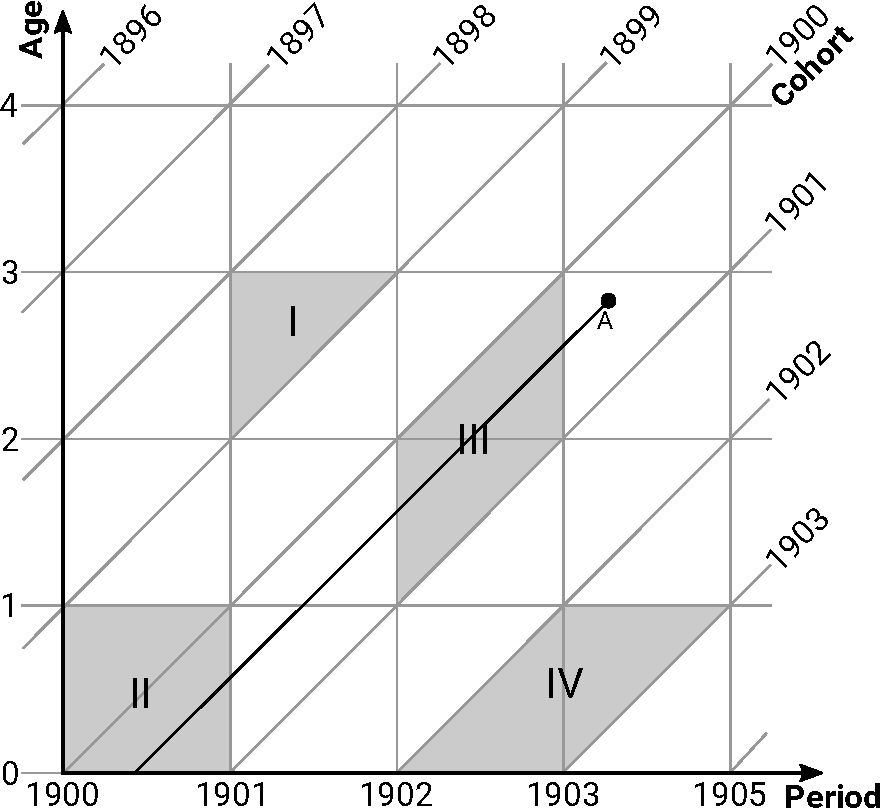
\includegraphics[width = 0.5\textwidth]{./fig/lexis_grid.pdf}
  \caption{The Lexis diagram.}
  \label{fig:lexis}
\end{figure}

% Populations on a Lexis diagram
Collecting data on many lifelines gives rise to the study of a population. In order to construct occurrence-exposure rates\footnote{
Events over person-years at risk.
}
and consequently lifetables individual lifelines and events are aggregated over some area of the Lexis diagram. A Lexis triangle marks an area specified by intervals over period, age and cohort, e.\,g.~everyone born in 1898 and dying in 1901 at the age of 2 (see figure~\ref{fig:lexis} shape I). Aggregating over intervals of period and age alone results in a rectangular region on the Lexis diagram, e.\,g.~everyone dying in 1900 at age 0 (see figure~\ref{fig:lexis} shape II). A parallelogram with vertical lines marks an area over a cohort and period interval, e.\,g.~everyone born in 1900 and dying in 1902 (see figure~\ref{fig:lexis} shape III), while a parallelogram featuring horizontal lines defines observations aggregated over a cohort and age interval, e.\,g.~everyone born in 1902 and dying at age 0 (see figure~\ref{fig:lexis} shape IV).

% The Lexis surface
The Lexis diagram as a mosaic of triangles, squares or parallelograms, each holding some aggregate statistic $z$, naturally connects to the Lexis surface as a visualization of population data across period and age.\footnote{
  \textcite{Arthur1984} introduce the term \enquote{Lexis surface} to describe a period-age plane of population densities. Subsequently it has been extended by \textcite{Vaupel1987a} to visualizations of demographic quantities on such a surface.
}
However, both tools have been developed independently. The earliest demographic surface plot is a perspective drawing of Swedish population counts by period and age published in 1860 and thus pre-dating Lexis' publication by 15 years (\cite{Caselli1990}). This graph was later redrawn and popularized by Luigi Perozzo (\cite{Perozzo1880}), still, it was not until the 20$^\text{th}$ century that surface plots gained traction in the demographic literature. The pioneers \textcite{Kermack2001} and \textcite{Delaporte1942} used contour lines to indicate regions of similar mortality levels and improvements on the period-age surface noting the emergence of regular patterns. \textcite{Vaupel1987a}\footnote{
  This publication has been facilitated by the work of \textcite{Gambill1985} who developed \texttt{LEXIS}, a plotting software for personal computers designed to produce shaded contour maps. Today these maps can be created by a wide range of software. In this paper we use the R language for statistical computing (\cite{R2016}) in conjunction with the \texttt{ggplot2} package (\cite{Wickham2016}) to plot the compositional Lexis surfaces.
} demonstrated the universal utility of period-age surfaces plotting a wide range of measures such as between country mortality rate ratios, population numbers, sex ratios, fertility rates or model residuals as shaded contours across period and age with darker colours indicating higher values. The same technique was used extensively by \textcite{Andreev1999} to demonstrate age-heaping over time in data on high age mortality and to describe the development of Danish mortality throughout the 18$^\text{th}$ and 19$^\text{th}$ century. Lexis surfaces have been sighted outside of demography as well: \textcite{Sula2012} used them to show how publication practices changed over historical time and the length of a researchers career. Though concerned with different phenomena, a unifying theme in all these references is the authors interest in \emph{period-, age-, and cohort effects}.

% age, period, and cohort effects
Take for example a surface of the mortality rate sex ratio in England \& Wales (see figure~\ref{fig:lexis_surface}). The excess male mortality resulting from military deaths during the first and second world war leaves a trail on the Lexis surface in the form two vertical bands of deep blue colour -- a classic example for a \enquote{period effect} where a cross-section of the population is affected by an historical condition. But we also see an interaction between period and age: The high levels of excess male mortality during the wars are limited to the age range of men in active military service. Starting in the mid-1950s we observe the emergence of excess mortality among young men. This age effect is visible as a horizontal corridor of deep blue colour and can be traced back to the effective prevention and treatment of infectious diseases which in turn put more emphasis on the more male dominated accidental deaths in early adulthood (\cite{Gjonca2005}). The diagonal colour pattern around ages 50--80 and years 1950--1980 marks a cohort effect and can be traced back to those born at the end of the 19$^\text{th}$ and the beginning of the 20$^\text{th}$ century. The rising popularity of smoking among men took its toll later in life in the form of lung-cancer. Women of the same cohorts smoked less than men and therefore gained a survival advantage. This advantage vanished once women took up smoking as well (\cite{Preston2006}; \cite{Beltran-Sanchez2015}).

% The Lexis surface
\begin{figure}[!htb]
  \centering
  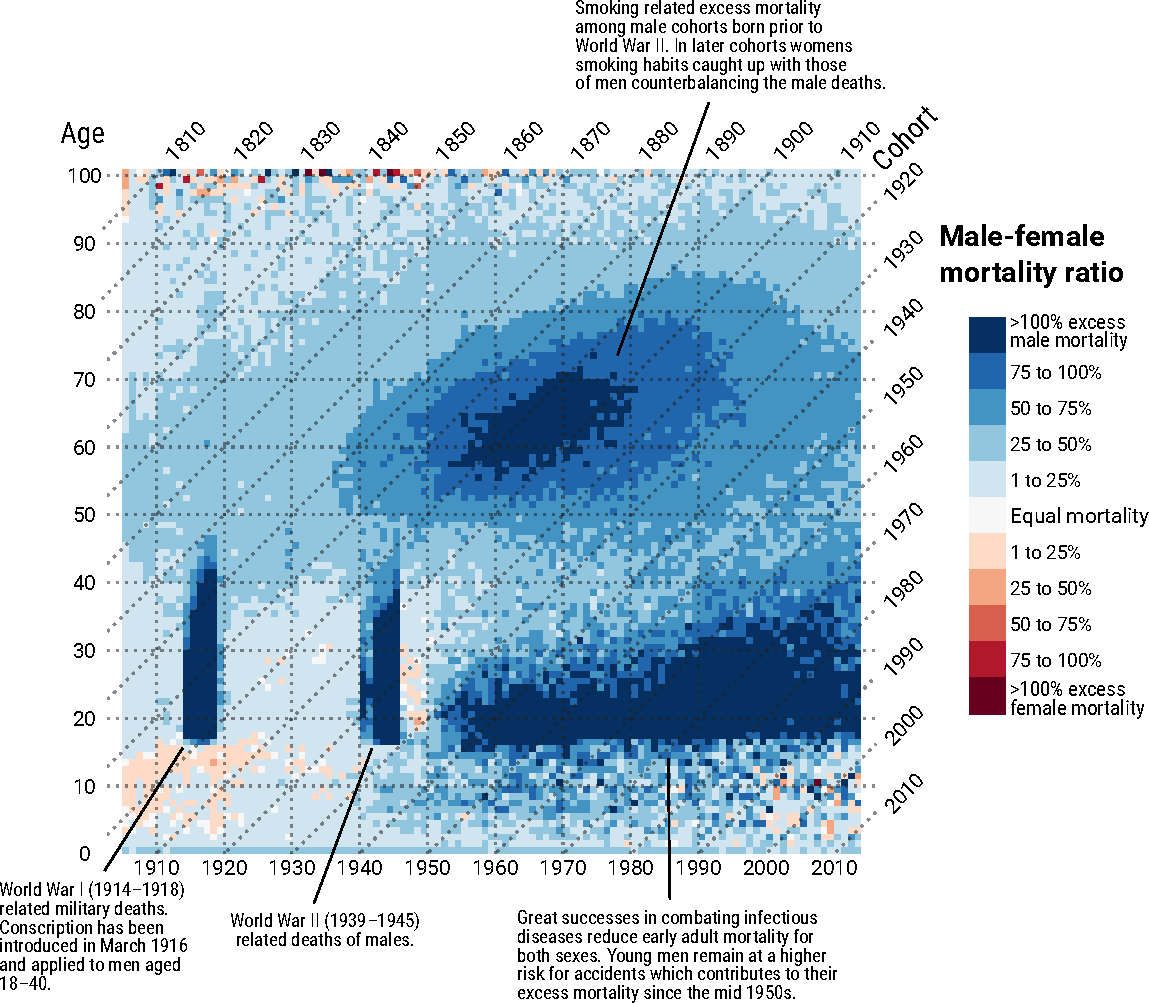
\includegraphics[width = \textwidth]{./fig/lexis_surface.pdf}
  \caption{The Lexis surface plot as a tool to identify age-, period-, and cohort effects. Ratio between male and female age-specific mortality rates in England \& Wales, 1841--2013. Data: Human Mortality Database, own calculations.}
  \label{fig:lexis_surface}
\end{figure}

In this paper we demonstrate the Lexis surface as a tool to explore the age-, period-, and cohort structure of \emph{compositions}.

\clearpage

\section{About colour} %%%%%%%%%%%%%%%%%%%%%%%%%%%%%%%%%%%%%%%%%%%%%%%%%%%%%%%%
\label{sec:colour}

% Section intro
We introduce colour as a multidimensional visual attribute, relate it to the display of compositional data and introduce the colour terminology used in this paper.

% Colour in visualizing compositional data
Why use colour to display compositional data on the Lexis surface?
  (1) Colour can be used to visualize the value of a third variable on a plane.
  (2) Colour is a visual attribute that is both inherently \emph{compositional} as well as \emph{multidimensional}. Each colour can be understood as a composition of primary colours mixed in certain proportions. The mixed colour itself is perceived as light or dark, pale or strong, tending to red, blue, or green. Two of our proposed techniques make use of these features: While the \emph{ternary-balance-scheme} employs the compositional nature of mixed colours to encode compositional data the \emph{qualitative-sequential scheme} maps perceptional colour dimensions to data dimensions.

% Primaries and colour mixtures
Children learn how to produce a wide range of colours by mixing blue, red and yellow paints. The resulting colour depends on the ratio among these \emph{primary colours}: Mix yellow with blue to produce green, red with blue to produce purple and three parts of yellow with one part of red to produce orange. In a case where every unique mixture of primaries resolves into a unique mixed colour one has effectively encoded a number of attributes (the proportions among the primary colours) into a single attribute (the mixed colour). Assigning a primary colour to each of three groups in the data and mixing the colours according to the proportions among the groups is the basic idea behind the ternary-balance-scheme (see appendix \ref{sec:app-tbs} for its construction).

% Perceptional colour dimensions
Another way to look at colour is in terms of perceptional features. When asked to describe a colour it would be a remarkable feast for a person to express it as proportions among primary colours. Instead one tends to say that a colour is dark or light (\emph{lightness}: \testclr{light1} \testclr{light2} \testclr{light3}), pale or pure (\emph{chroma}: \testclr{chroma1} \testclr{chroma2} \testclr{chroma3}), and tending to red, blue, green\ldots (\emph{hue}: \testclr{hue2} \testclr{hue3} \testclr{hue1}).\footnote{
  See \cite{Fairchild2005} chapter 4 for an introduction to colour terminology.
}
This specification is widely used in visualization research as it allows for the construction of \emph{colour schemes} which reflect the statistical features of the variables one wishes to visualize: Lightness and chroma are perceived as ordered attributes, e.\,g.~a random sequence of lightness or chroma steps can easily be arranged from dark to light, from pale to pure. Both dimensions therefore lend themselves to the display of ordered data such as proportions (0\,\%~\testclr{light3} \testclr{light2} \testclr{light1}~100\,\%). Different hues on the other hand do not imply order and therefore signify mere categorical difference (blueberry~\testclr{hue3} \testclr{hue1}~cherry). Based on this connection \textcite{Brewer1994} proposes a typology of colour schemes: The \emph{sequential} and the \emph{qualitative} scheme encode ordered and categorical data respectively. Crossing both leads to the \emph{qualitative-sequential scheme} -- a bivariate colour scheme encoding the order and the category of a data point (see figure~\ref{fig:brewer} for an illustration of the Brewer schemes employed in this paper).

% brewer schemes
\begin{figure}[!htb]
  \centering
  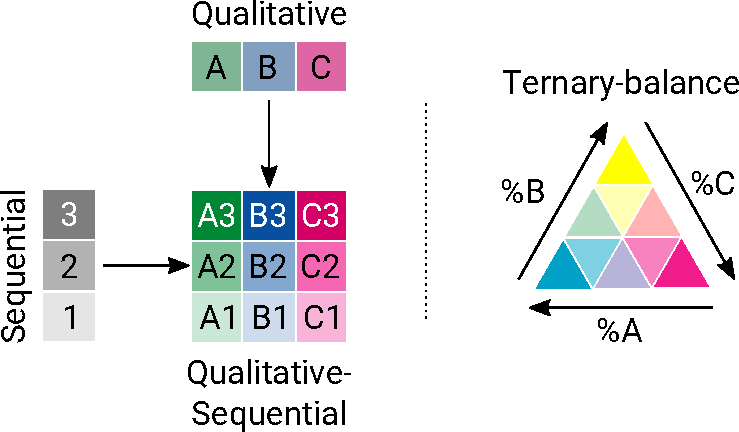
\includegraphics[width = 0.5\textwidth]{./fig/brewer_subset.pdf}
  \caption{Colour schemes used in this paper (derived from an illustration in \cite{Brewer1994}).}
  \label{fig:brewer}
\end{figure}

\clearpage

\section{Ternary-balance-scheme} %%%%%%%%%%%%%%%%%%%%%%%%%%%%%%%%%%%%%%%%%%%%%%
\label{sec:tbs}

\begin{figure}[!htb]
  \centering
  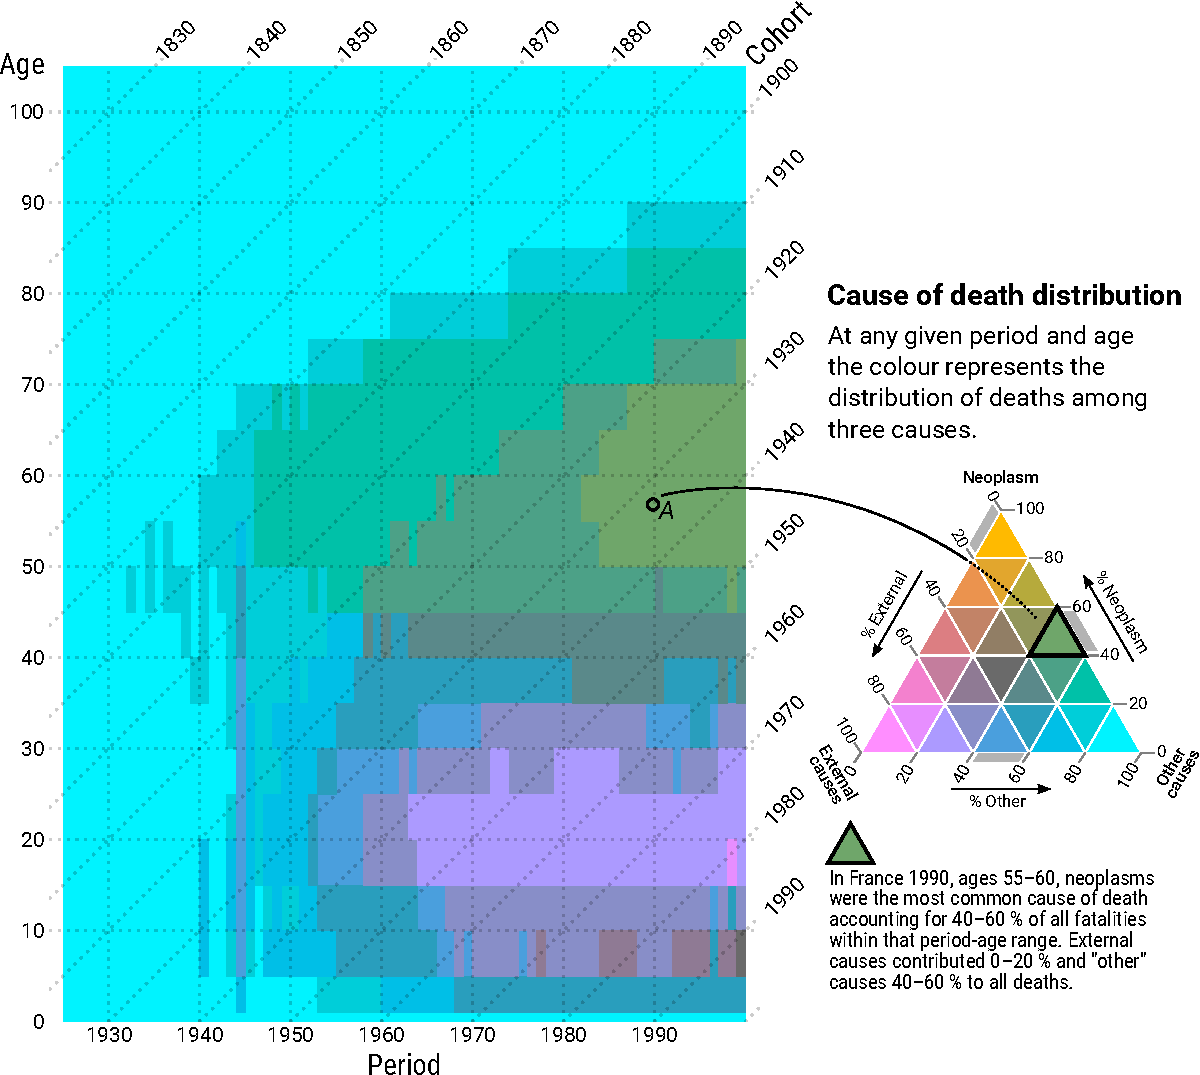
\includegraphics[width = \textwidth]{./fig/tern_balance.pdf}
  \caption{The ternary-balance-scheme technique applied to French cause of death data. Age specific proportions of of people dying from a given cause in France 1925--1999, total population. Data: \cite{Vallin2014}, own calculations.}
  \label{fig:tbs}
\end{figure}

% Ternary-balance-scheme
The idea behind the \emph{ternary-balance-scheme} is to represent the proportions among three groups as a mixture of three basic colours each corresponding to a single group. The basic colours are chosen so that their hues are dissimilar to each other (e.\,g. magenta, yellow, cyan). They are then mixed in proportions given by the group composition. The resulting colour mixture is unique for every possible combination of proportions among three groups as can be shown in a colour-coded ternary diagram serving as a legend for the ternary-balance Lexis surface.\footnote{See appendix~\ref{sec:app-tbs} for details on the construction of the ternary-balance colour scheme.}

% Critique of multivariate colour scales
While using colour mixtures to encode multiple data dimensions in a single point has been proposed several times\footnote{
  See for example \textcite{Trumbo1981} and \textcite{Eyton1984} for bivariate data on geographical maps and \textcite{Ware1988} for cluster identification in high-dimensional spaces.
}
such techniques are not in widespread use, possibly due to the usage of legends which are not easily memorized (\cite{Wainer1980}). We seek to alleviate these issues by providing straightforward interpretation guidelines along with a legend that builds upon an already established tool in compositional data analysis -- the ternary diagram.

% Interpreting the Ternary-balance-scheme
The dominant group at any point in time as well as the overall distribution of the group proportions can be understood keeping two principles in mind:

\begin{compactenum}
  \item The higher the proportion of a group, the more the mixed colour resembles the base colour for that group, and
  \item the more balanced the proportions among the groups, the more the mixed colour tends to grey.\footnote{
  To enable a proper differentiation between the colours we added a lightness contrast in addition to the chroma contrast so that more balanced compositions are represented by darker colours. See appendix \ref{ssec:lboost} for further details and a comparison of ternary-balance-schemes with and without lightness contrast.
  }
\end{compactenum}

The ternary diagram as legend colour codes all possible proportions among three groups in a structured way so that each point on the Lexis surface can be decoded into its precise proportions if needed.

Figure \ref{fig:tbs} shows the ternary-balance-scheme applied to agewise French cause of death data across the $20^\text{th}$ century. All deaths are divided by cause into the categories \enquote{Neoplasm} (ICD-9 codes 140--239), \enquote{External} (injury, suicide, accident; ICD-9 codes 800--999 and E--V) and \enquote{Other} (all remaining causes of death). Magenta was chosen as a primary colour for external causes of death, orange for death by neoplasm and cyan encodes all remaining deaths.

\textsc{Example:} Consider point \emph{A} in figure~\ref{fig:tbs}. The proportion of deaths caused by neoplasm is given in the legend by the position on a horizontal line through the region with the colour of \emph{A}; likewise the proportion of deaths caused by external causes is indicated by the position on a \textbackslash~line and and the proportions of all other causes is indicated by the position on a /~line. The mixture of magenta, orange and cyan at point \emph{A} indicates that 40 to 60\,\% of the deaths among persons of ages 55--60 in 1990 were caused by neoplasms, 0 to 20\,\% by external causes and the remainder of 40 to 60\,\% by all other causes of death.

The mid-century marks a turning point. Prior to 1950 external causes of death and cancer were only sporadically found on the death certificates the prominent exception being World War II. Period effects are visible in 1940 when Germany occupied France and -- much stronger -- in 1944 after the Allied landing in the Normandy. In both years the war contributed deaths by external cause as visible in the age range 5--60. After 1950 two major trends in the distribution of death causes emerged:
  (1) Adolescent deaths rapidly became dominated by external mortality, and
  (2) deaths due to cancer gradually became more common in the age range 40--80, dominating the ages 50--70 since the 1980. The onset-age of \enquote{other} causes of death as the most prominent increased along the cohort diagonal.

% Pros and Cons
The ternary-balance-scheme technique allows us to identify major patterns in the change of group composition over period and age. We are able to identify symmetrical mixtures as well as clear monopoles among groups. Age-, period- and cohort-effects look much like they would on a conventional Lexis surface of all-cause mortality rates: Local outliers show up as a sharp shift in hue -- vertical for period effects, horizontal for age effects and on a $45^{\circ}$ slope for cohort effects. Slower transitions are marked by gradual shifts in colour.\footnote{
  Figure~\ref{fig:tbs_cont} shows the French cause of death data visualized using a \emph{continuous} ternary-balance-scheme which is especially well suited for showing gradual changes in composition. It also works well with super-imposed contours of overall mortality rates, displaying not only composition but also magnitude of mortality across period and age. A discrete scale as used in figure~\ref{fig:tbs} however has the advantage of pronouncing existing patterns in the data by introducing sharp contours between regions of different colours. Reducing the number of colours in the ternary scale also makes it easier to relate a colour on the plot to a colour in the legend. In appendix \ref{ssec:disc} we describe how to discretize a continuous ternary composition into $N$ equally sized regions on a ternary diagram.
}
The obvious drawback of the ternary-balance-scheme is the limitation to three distinct groups. Also, using colour as a quantifier, small changes in the values are hard to detect and the very nature of the graph makes it unsuitable to use for people with impaired colour-vision.

\clearpage

\section{Qualitative-sequential-scheme} %%%%%%%%%%%%%%%%%%%%%%%%%%%%%%%%%%%%%%%
\label{sec:qss}

\begin{figure}[!htb]
  \centering
  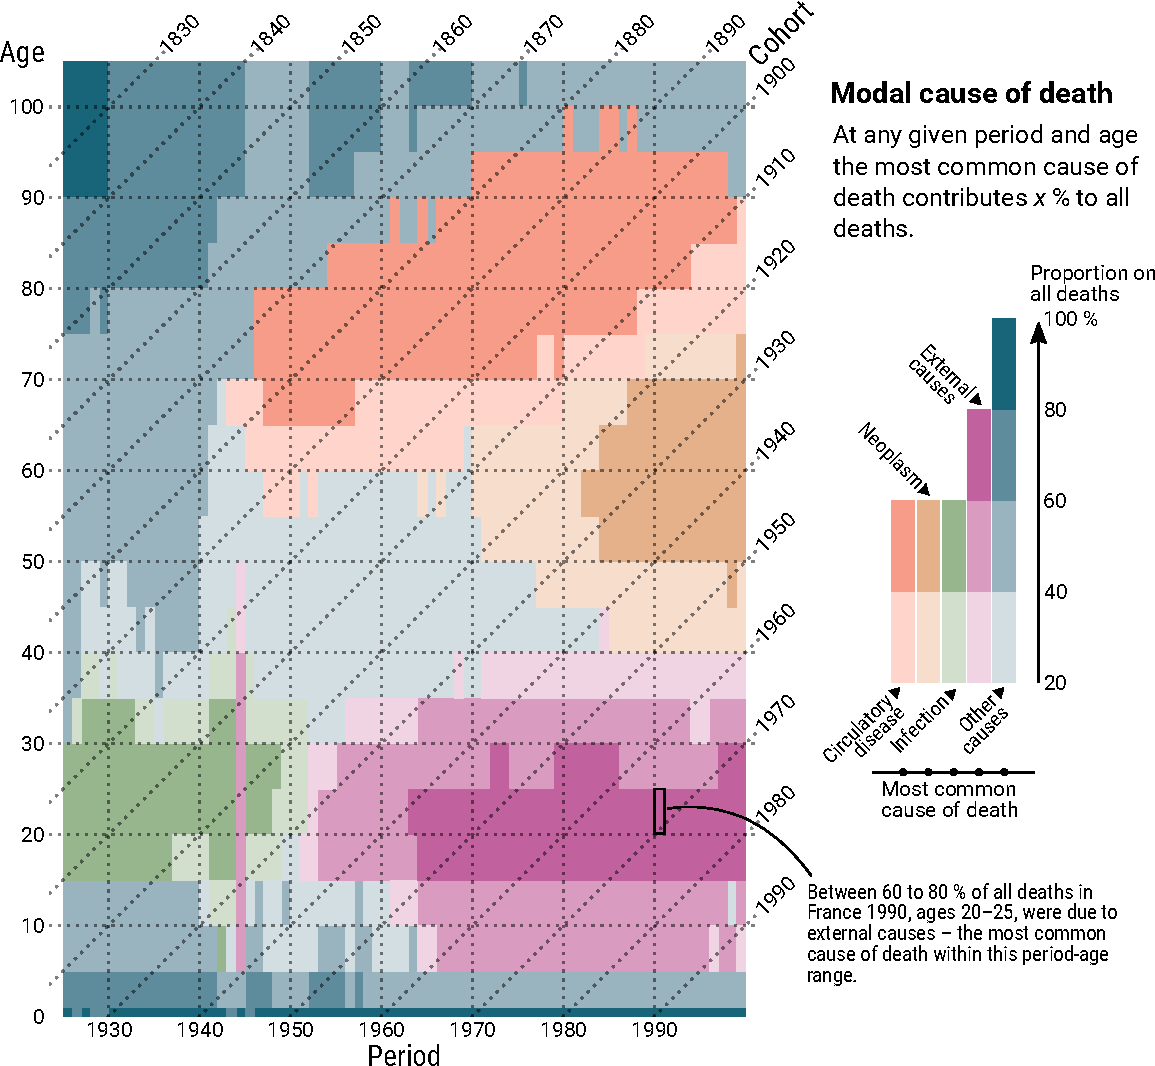
\includegraphics[width = \textwidth]{./fig/qual_seq.pdf}
  \caption{The qualitative-sequential-scheme technique applied to French cause of death data: The most common cause of death by period and age and its proportion on all deaths in France 1925--1999, total population. Data: \cite{Vallin2014}, own calculations.}
  \label{fig:qss}
\end{figure}

% Qualitative-sequential-scheme
Another form of multivariate colour scheme is the qualitative-sequential-scheme (\cite{Brewer1994}). The idea is to use a qualitative palette of different hues to signify group-membership and to construct a sequential palette for every group by varying the lightness of the group-colour and thereby encoding group-specific quantities.

See figure~\ref{fig:qss} for an example using the same dataset as in figure~\ref{fig:tbs} but with two additional categories, namely death due to infectious diseases (ICD-9 codes 001--139) and diseases of the circulatory systems (ICD-9 codes 390--459). Each group is assigned its own sequential colour scheme. The values given by the colours on the Lexis surface represent the proportion of deaths from the most prominent cause of death at period $t$ and age $x$.

This approach allows to account for more than three groups in the composition. The downside is an incomplete picture for every point on the Lexis surface: Only information on the group with the highest proportion is given. However, in a dataset with a lot of variation in the group proportions interesting patterns emerge.

\textsc{Example:} Consider age group 60--65 in figure~\ref{fig:qss}. Prior to 1945 we see a blue colour: \enquote{other} causes of death were dominant. This dominance subsequently declined (a lighter blue) until, post World War II, circulatory diseases became the main cause of death with a proportion on all deaths of 20--40\,\%. Around 1970 the main cause of death shifted from circulatory diseases to neoplasms (the hue shifts from red to yellow). The dominance of neoplasms over other causes of death for 60--65 year old males and females increased with time (the yellow hue gets darker and more saturated).

One new insight this visualization yields is the importance of infectious diseases as a cause of death for people aged 15--40 prior to 1950. In these years and ages 20--60\,\% of the deceased died from infection making this the most likely cause of death in adolescence and middle-age. The pattern abruptly changed after 1950 with external causes of death taking the top spot. Similar to figure~\ref{fig:tbs} we see the proportion of accident mortality on all deaths peaking around ages 15--30.

We also get a more differentiated picture concerning causes of death in old age which is dominated by failures of the circulatory system. Over time the onset of circulatory conditions as the main cause of death moved into higher ages starting at around age 60 in the 1940s to age 75 in the 1990. For people with an extraordinarily long lifespan the causes of death are more diverse with the group \enquote{other} in the lead.

% Pros & Cons
While confined to visualize proportions only for the most prominent group at any given point on the Lexis surface, the qualitative-sequential scheme still reproduces a lot of the information gained from figure~\ref{fig:tbs} while adding new insights. In cases where the dominant group does not change along the surface, this style of visualization loses its appeal.

\clearpage

\section{Agewise-area-plot} %%%%%%%%%%%%%%%%%%%%%%%%%%%%%%%%%%%%%%%%%%%%%%%%%%%
\label{sec:aag}

\begin{figure}[!htb]
  \centering
  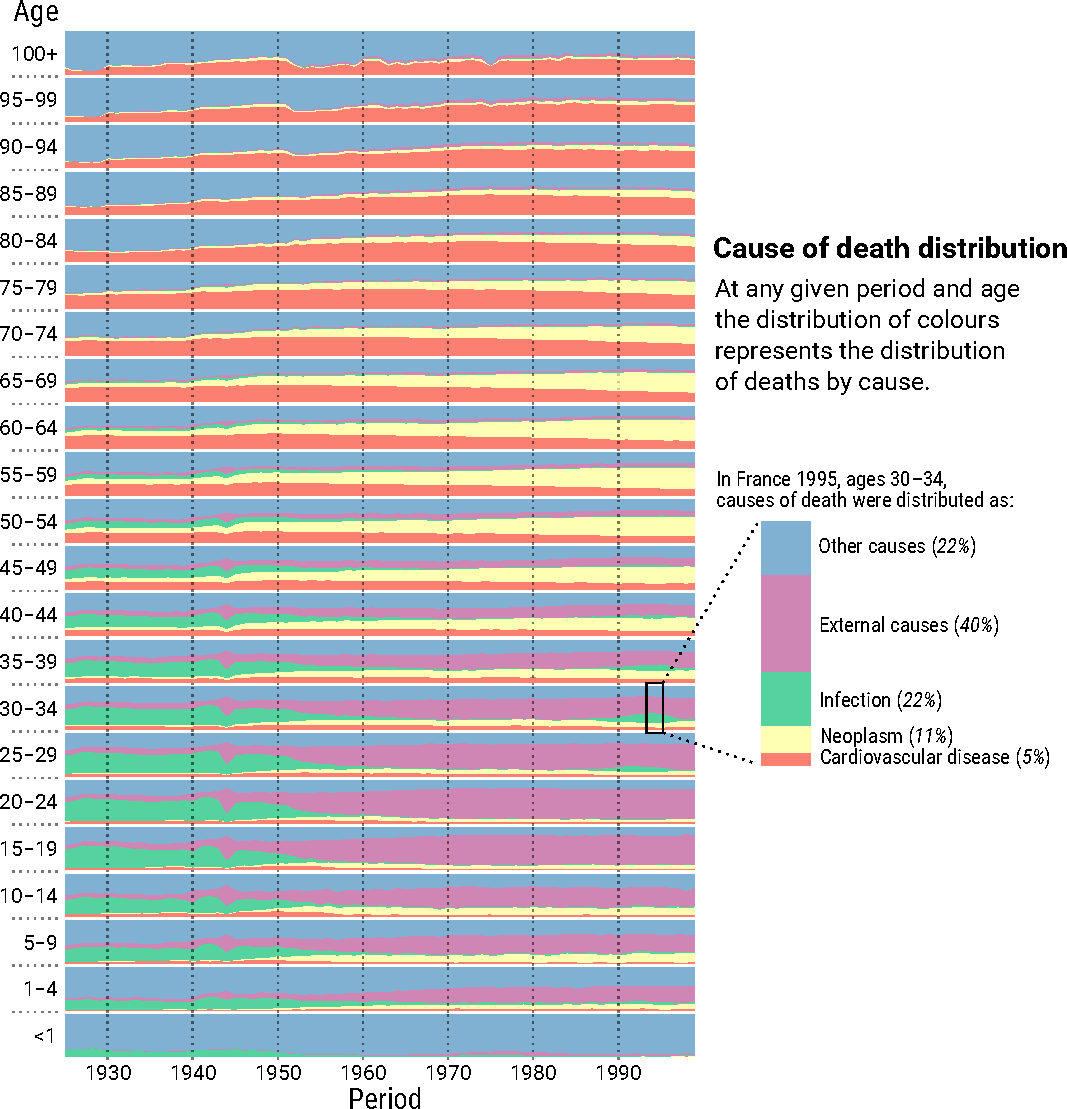
\includegraphics[width = \textwidth]{./fig/agewise_area.pdf}
  \caption{The agewise-area technique applied to French cause of death data: Age specific proportions of of people dying from a given cause in France 1925--1999, total population. Data: \cite{Vallin2014}, own calculations.}
  \label{fig:aag}
\end{figure}

% Agewise-area-graph
The \emph{stacked-area-plot} can be thought of as the continuous version of a stacked-bar-chart. Coloured areas indicate group proportions which change along the $x$-axis. As the value of each individual group proportion is indicated by length as opposed to colour this technique is better suited to detect slight changes in group composition over time than the previous approaches. \textcite{Cleveland1984} show that people decode visual information into their numerical equivalents (\emph{table look-up}) more easily when it is represented by length and not by colour.

For the \emph{agewise}-area-plot (see figure~\ref{fig:aag}) we produce the stacked-area-chart separately for every age group and assemble all of them on a Lexis-like grid. Unlike with the ternary-balance-scheme technique we are able to distinguish more than three groups and unlike with the qualitative-sequential-scheme technique the full information about the composition is displayed.

\textsc{Example:} One feature of the data which was hidden by the former graphical representations is the unusual surge of fatal infectious diseases during the 1990s around ages 25--45. Looking at the exact cause of death data we see that HIV related deaths are the reason for this local phenomenon. Another new insight from this plot is the relative importance of cancer as a cause for childhood mortality.

% Pros & Cons
The plot does not show a true Lexis surface. The period-age grid is \emph{non-continuous} as it is composed of multiple stacked-area-charts each having a separate $y$-axis ranging from 0\,\% to 100\,\%. This breaks the plot area into separate sections making the perception of global patterns harder because the global graphical patterns (the shape of the equal-colour areas across period and age) are interrupted along the age-scale.

The strength of the agewise-area-plot is the clear display of small local phenomena and developments within single age groups while still giving an overview of the global patterns for multiple groups on a single period-age grid.

\clearpage

\section{Small-multiples} %%%%%%%%%%%%%%%%%%%%%%%%%%%%%%%%%%%%%%%%%%%%%%%%%%%%%
\label{sec:sm}

\begin{sidewaysfigure}[!htb]
  \centering
  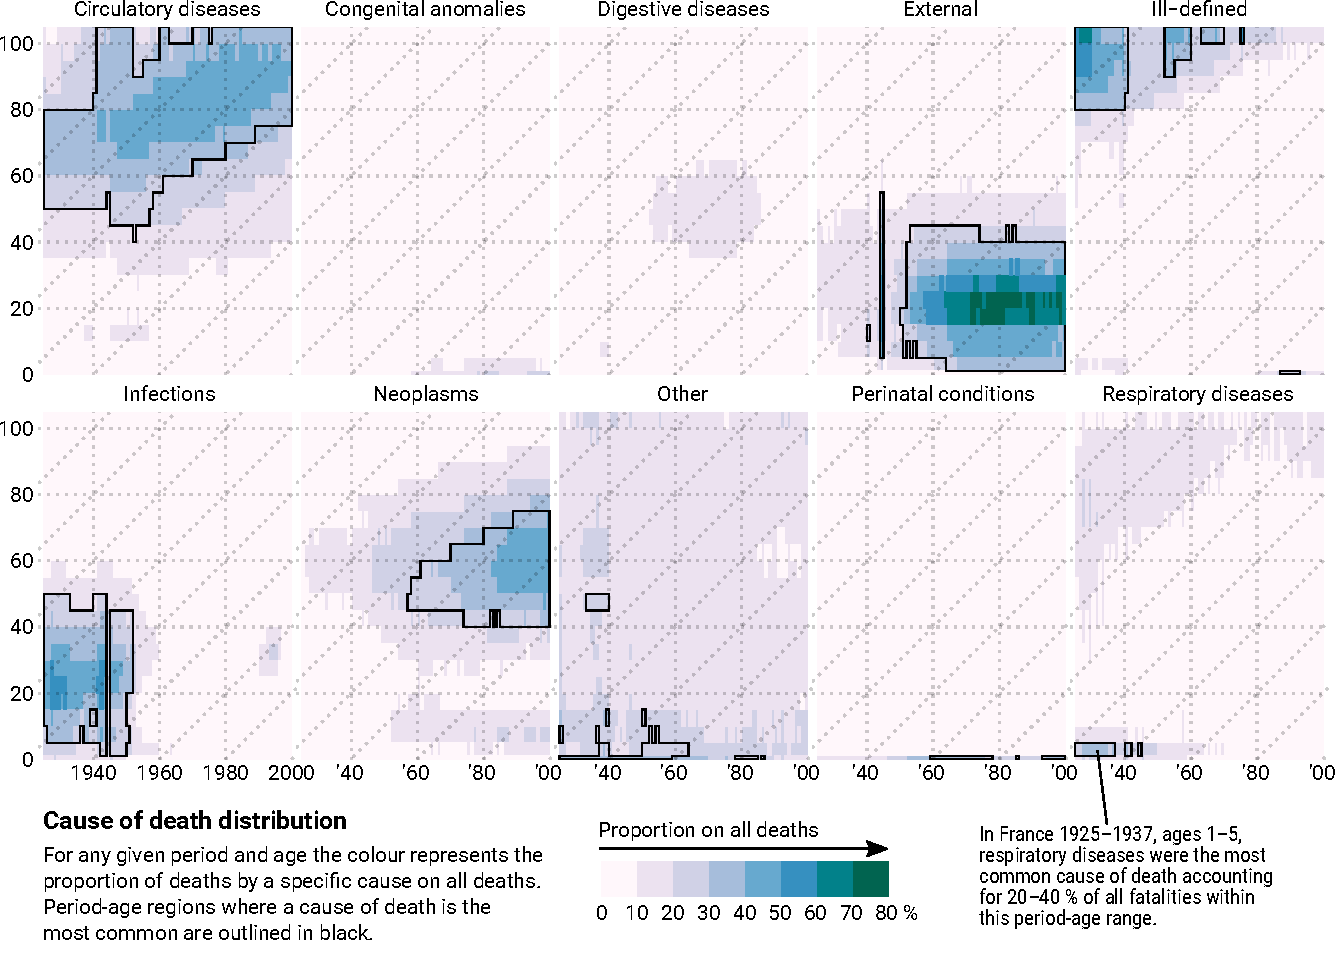
\includegraphics[width = \linewidth]{./fig/small_multiples.pdf}
  \caption{The small-multiples technique applied to French cause of death data: Age specific proportions of of people dying from a given cause in France 1925--1999, total population. Data: \cite{Vallin2014}, own calculations.}
  \label{fig:smg}
\end{sidewaysfigure}

% Small-multiples
\emph{Small-multiples}\footnote{
  We use the terminology of \textcite{Tufte1990}. Closely related concepts are \emph{facets} (\cite{Wilkinson2005}) or \emph{trellis-plots} (\cite{Becker1996}).
}
are \enquote{tables of graphs} (\cite{Wilkinson2005}:319). Each panel within the table represents a level of a categorical variable or an interaction level among multiple categorical variables. Small-multiples are a fairly common technique and have already been discussed by \textcite{Vaupel1987a} as a way of plotting Lexis surfaces for multiple sub-populations. We discuss this technique in the context of compositional data and propose a small adjustment facilitating cross-panel comparisons.

In figure~\ref{fig:smg} we see multiple Lexis surfaces displaying cause-specific proportions of deaths in France across period and age. The plots are augmented by border lines around regions within a given cause of death is dominant.

\textsc{Example:} Consider the lower left panel. It shows the proportion of deaths caused by infectious diseases by age and calendar time. Point \emph{A} indicates that in 1930 infectious diseases are the dominant cause of death for persons aged 30--34 with 40--50\,\% of all deaths caused by infection. Around 1950 external causes start to become the dominant cause of death for persons aged 1--40, increasing their proportion within that age range over time.

% Pros & Cons
Unlike the other visualization techniques described in this paper the small-multiples allow us to display the cause of death proportions among each of the 10 most prominent categories of ICD-9. This power of course comes with a price: The data is not contained in a single graphic. This means that the eye (and the mind) not only have to move between and compare different regions of a plot but make connections between different graphics in order to \emph{grasp the whole picture}. To make these comparisons easier we use black outlines to distinguish regions on the period-age surface in which the corresponding cause of death has the highest proportion among all deaths. This way there is no need for cross-panel comparisons in telling if a given cause of death dominates over all other at some point on the Lexis surface.

Yet again the new visualization technique shines a different light on our data and allows for additional insights. We can see that causes of death in old age are frequently not known: Prior to World War II an ill-defined cause of death was the norm for people dying at ages 80+. Perinatal conditions followed by congenital anomalies were the main causes of death for infants through most of the 20$^\text{th}$ century in France. Prior to 1950 deaths of infants and young children have, for the most part, been attributed to respiratory diseases. For adults fatal respiratory diseases move into higher and higher ages, reaching a plateau around 1970 and being nearly exclusively an old-age phenomenon from there on. A period-age effect can be identified in the realm of digestive diseases which contributed more than 10\,\% of all deaths during the period 1960--1980 in ages 40--60. The latter half of the 20$^\text{th}$ century sees a rise in the proportion of people aged 35--65 dying from conditions of the digestive system. However, note that the data is binned into 10\,\% categories simplifying a correct look-up of the colour values but forbidding the exact judgement of small differences.

\clearpage

\section{Comparative evaluation} %%%%%%%%%%%%%%%%%%%%%%%%%%%%%%%%%%%%%%%%%%%%%%
\label{sec:eval}

In this section we evaluate and compare the four proposed techniques along the criteria completeness, continuity, group limit, pattern perception, table look-up, colour accessibility, and footprint.

% Completeness
\begin{description}
  \item[Completeness] is the question whether or not all values of the compositional data (e.\,g.~all individual group proportions for each period-age) are displayed in the visualization or if only a subset of the group data (e.\,g.~the proportion of the largest group for each period-age) is visualized. Visualising the complete dataset is desirable during exploratory data analysis.
\end{description}

If the visualization must contain complete information on every group in the composition the qualitative-sequential-scheme technique is not an option as only the group with the highest proportion at a given period-age is considered. The remaining three techniques always show the complete distribution of proportions.

% Continuity
\begin{description}
  \item[Continuity] requires that the continuity of the Lexis grid is preserved in the visualization, e.\,g.~the period and age axes constitute a rectangular grid unbroken by whitespace or period-wise/age-wise scales.
\end{description}

The Lexis surface constitutes a continuous grid of period and age. The agewise-area-plot breaks this essential feature by fracturing the surface into separate plots by age. As each age group uses its own $y$-axis the surface becomes discontinuous along the age dimension. From a perceptional standpoint this hinders the identification of period- and cohort effects as these would form continuous patterns along the vertical or diagonal of the plot area but cannot do so in the agewise-area-plot. This is not an issue for the remaining visualization techniques.

% Group limit
\begin{description}
  \item[The group limit] describes how many groups in the composition can be accommodated by a given technique. It is precise if limited by technical reasons or approximate if limited by perceptional reasons.
\end{description}

The ternary-balance-scheme technique, as the name suggests, only allows for the display of proportions among three groups. Opposed to that the small-multiples approach allows for the simultaneous display of a virtually unlimited number of group proportions.

The group limit of the qualitative-sequential-scheme and the agewise-area-plots is not restricted by technical- but by perceptional limits. The qualitative-sequential scheme uses lightness steps within different hues to show different group proportions. Therefore the number of groups which can sensibly be displayed at once is limited by the number of hues one can differentiate across varying lightness steps. \textcite{Ware2013} lists four \emph{unique} hues: red, green, blue and yellow. These hues are are generally perceived as pure/unmixed colours which do not resemble each other. Yellow is problematic as a base hue for a lightness sequence as it is already a very light colour (\cite{Ware2013}:127). Orange, still being perceived distinct from red and yellow, is the better choice here. Adding black one can construct five sufficiently different lightness sequences. Some few additional hues, like purple, might also work.

The agewise-area-plots contain a lot of information in a small vertical space. The more groups are added, the more crowded this vertical space gets and information retrieval will be more difficult.

% Pattern perception
\begin{description}
  \item[Pattern perception] describes the \enquote{visual decoding of physical information} (\cite{Cleveland1994}:223\,f). Within the context of our paper this translates into the degree at which age-, period-, and cohort effects in the composition of the data are revealed by the visualisation.
\end{description}

The ternary-balance-scheme, the qualitative-sequential-scheme and the small-multiples techniques all show colour on a continuous surface and differ only in the applied colour scheme. They are particularly suited to show patterns in the data such as period-, age- and cohort-effects or local outliers (as demonstrated for 1-dimensional data in \cite{Vaupel1987a}). However, for the small-multiples approach this merit only applies to each group on its own as the visualization is spread out across multiple panels -- the inter-group patterns are not directly visually encoded and have to be inferred from a comparison between multiple panels. The marking of modal values eases this task.

The case for agewise-area-graphs is more complicated. Due to the discontinuities across the age dimension the global pattern-perception from these graphs is comparatively worse, though changes over time within single age groups, even small ones, can be seen very well using this approach.\footnote{
  Given that no steep slopes occur or else there will be problems correctly judging the difference between the upper and lower boundary of an area -- the value (\cite{Cleveland1994}:227\,ff).
}

% Table look-up
\begin{description}
  \item[Table look-up] \enquote{[is the] visual decoding of scale information [\ldots]} (\cite{Cleveland1994}:223\,f). It takes place when attempting to extract the exact numbers from a displayed data point. Some visual primitives (such as xy-position, height, size etc.), and therefore some visualizations, make this task easier than others. Being able to easily decode the data values from a visualization is desirable as it allows for numerical statements (e.\,g.~\enquote{A is 2.5 times higher than B}).
\end{description}

None of the discussed techniques allows for a very efficient table look-up operation, i.\,e.~the quick and accurate retrieval of the underlying data values. Colour, as used by three out of the four techniques as encoding for the group proportions, is generally regarded as the weakest graphical element in terms of table look-up (\cite{Cleveland1984}). The judgement of areas and lengths as used in the agewise-area-plots fares better. For the bottom group the value can be directly read from the y-axis. For all other areas, differences between two points on the y-axis equal the data value.

% Colourblind safeness
\begin{description}
  \item[Colour accessible] visualizations can be read by people with impaired colour vision. Most forms of colour blindness affect the ability to discriminate between red and green hues. In Europe the prevalence of inherited red-green colour deficiency is estimated to be around 8 percent among males and less than a percent among females (\cite{Birch2012}). Accessible colour palettes avoid red-green contrast and use lightness contrasts to make the colours distinguishable for people with impaired colour vision. Varying the lightness between colours also improves the legibility of the visualization when printed out in grey scale.
\end{description}

Only the small-multiples technique is truly accessible as it does not rely on differences in hue to encode information but rather uses a sequential colour scale with a strong lightness gradient to express the data. This makes small-multiples the number one choice if the plot is to be read in grey scale or by people with impaired colour vision. The ternary-balance-scheme on the other hand is inherently unsuited in that regard relying heavily on the ability to distinguish a wide range of hues from each other. The same goes for the qualitative-sequential scheme which uses hue and lightness as independent channels mapped to different variables. It can not be reproduced in grey scale without losing information and will be difficult or impossible to read if colour vision is impaired as one must correctly identify hues across different lightness steps. A simple qualitative colour scheme is used in the age-wise-area chart and one can choose among the many available palettes designed with colour impaired users in mind.\footnote{See for example the web-application \emph{Colorbrewer} (\cite{Brewer2016}) for a choice of colourblind safe palettes.} Still, a reproduction in grey scale will make it harder to connect the shades of grey to their labels -- an issue which can be resolved by using direct annotation.

% Footprint
\begin{description}
  \item[The Footprint] is often of concern when publishing results. Some visualizations gain their descriptive power by occupying a large area.
\end{description}

The footprint of all techniques but the small-multiples is equal to a conventional Lexis surface plot across the same period-age-range. The small-multiples technique, depending on the number of groups, might be much larger up to the point of filling the whole page.

\begin{table}[!htb]
\tabformat
\begin{tabular}{p{3.5cm}*5{Q{1.5cm}}}
\toprule
 & Ternary-balance-scheme & Qualitative-sequential-scheme & Agewise-area-plot & Small-multiples \\
\midrule
Completeness & yes & no & yes & yes \\
Continuity & yes & yes & no & yes \\
Category limit & 3 & $\approx$ 5--6 & $\approx 8$ & unlimited \\
Pattern perception & good & good & limited & good \\
Table look-up & limited & limited & limited & limited \\
Colour accessible & no & no & yes & yes \\
Footprint & small & small & small & large \\
\bottomrule
\end{tabular}
\caption{Evaluation of different visualization techniques for compositional data on the Lexis surface.}
\label{tab:eval}
\end{table}

\clearpage

\section{Conclusion} %%%%%%%%%%%%%%%%%%%%%%%%%%%%%%%%%%%%%%%%%%%%%%%%%%%%%%%%%%
\label{sec:con}

We demonstrated four different visualization techniques for showing cause of death compositions across period and age, extending the conventional period-age Lexis surface of 1-dimensional continuous data (e.g. surfaces of mortality rates) to compositional data. We applied multivariate colour schemes originating from cartography to the Lexis surface (ternary-balance-scheme, qualitative-sequential-scheme), introduced agewise area plots as a means of visualizing compositional change over time within ages and improved upon the well known small-multiple technique in the context of compositional data. Each of these techniques serves the cause of making sense of compositional data across period and age, while at the same time these techniques complement each other by differing in their strong points.

The ternary-balance-scheme technique is the best candidate for visualizing the \emph{proportions among three groups}. Using colour composition it produces smooth rainbow-like surfaces immediately indicating period-, age-, and cohort patterns in the data. The qualitative-sequential-scheme technique \emph{extends beyond three groups} and shows the proportions of the most dominant groups on a surface. The agewise-area-plots use the power of the line to point out \emph{slight, age-specific changes} in group composition over time. Drawing a separate Lexis surfaces for each level of a categorical variable is a well-tried technique and still the most practical way to plot compositions featuring a \emph{large number of groups}. Adding an outline to each panel, indicating the regions of dominance of one group over the others, reduces the need for cross-panel comparisons and therefore further adapts this proven technique to the display of compositional data.

What proportion of a population features attribute $i$ at period $t$ and age $x$? The proposed visualizations are tools helping to answer this question. We demonstrated the techniques using data on causes of death. Other possible applications include period-age surfaces of population proportions by labour-market status (unemployed and seeking job, unemployed and not seeking job, employed), distributions of labour force over industries (agricultural, industry, service) or partnership status (single, in relationship and living alone, in relationship and cohabiting, married). The visualizations can also help interpreting the output from estimated models. The Heligman and Pollard model of overall mortality by age (\cite{Heligman1980}) for example is written as the sum of childhood-, accident- and senescent mortality by age. The relative magnitudes of these components can be clearly visualized using the ternary-balance-scheme, producing graphics of quasi cause-specific-mortality from all cause mortality data.

Good visualizations can be thought of as a visual model of the data at hand, able to identify relationships between variables. They go hand in hand with mathematical models of the data as both can be checked against the other. We hope to have contributed useful techniques for revealing information about compositions across time and age.

\clearpage

\section{Acknowledgements} %%%%%%%%%%%%%%%%%%%%%%%%%%%%%%%%%%%%%%%%%%%%%%%%%%%%
\label{sec:ack}

The authors would like to thank \emph{Anna Klabunde} and \emph{Katharina Wolf} of the Max Planck Institute for Demographic Research for their helpful comments on the paper, and \emph{Anja Schöley} for editing the draft.

\clearpage

%%%% Bibliography %%%%%%%%%%%%%%%%%%%%%%%%%%%%%%%%%%%%%%%%%%%%%%%%%%%%%%%%%%%%%

\sloppy
\printbibliography

\clearpage

%%%% Appendix %%%%%%%%%%%%%%%%%%%%%%%%%%%%%%%%%%%%%%%%%%%%%%%%%%%%%%%%%%%%%%%%%

% appendix figures follow A1, A2, B1... scheme
\renewcommand\thefigure{\thesection.\arabic{figure}}
\setcounter{figure}{0}

\begin{appendix}

\section{Construction of the ternary-balance-scheme} %%%%%%%%%%%%%%%%%%%%%%%%%%
\label{sec:app-tbs}

\subsection{The ternary-balance-scheme in the CIE-Lch colour space} %%%%%%%%%%%
\label{ssec:app-cie}

In the ternary-balance-scheme the colour mixture $\mathscr{M}$ of three primary colours encodes the proportions within a three element compositional vector $\textbf{p}$ (a ternary composition) with components $\langle p_1, p_2, p_3 \rangle \in \mathbb{R}_{\geq 0}^{3} | p_1+p_2+p_3 = 1.$ The mixture is computed as a convex combination (a weighted average) of the three primaries with weights determined by $\textbf{p}$.

There are multiple ways to construct such a ternary-colour mixture. We derive it from within the \emph{CIE-Lch} colour space because
  (1)~it is parametrized in terms of the perceptual colour dimensions lightness $l$, chroma $c$ and hue $h$,
  (2)~its parameters are uncorrelated with each other, and
  (3)~the colour space is \emph{perceptually uniform}\footnote{
  Colours specified as having the same lightness, hue, chroma will actually be perceived as equal in the respective dimensions. Furthermore, changes in the parameters of the colour space roughly correspond in magnitude to changes in the perceived colour predicted by the colour space. This property supports a truthful visual representation of the data at hand where similar compositions will be represented by similar colours and likewise dissimilar compositions by dissimilar colours (cp.~\cite{Ware2013}:105).
}.
These features give us great control over the final look of the ternary-colour-scheme.

The geometry of CIE-Lch can be thought of as a cylinder with different hues along the circumference, decreasing chroma along the radius towards the centre and increasing lightness along the vertical axis (cp.~\cite{Fairchild2005}:185\,ff.). Figure \ref{fig:cielch} shows a \enquote{slice} of this cylinder with a fixed lightness level.

Let $l$ be fixed at some $l^*$ between 0 (black) and 100 (white). Each colour within that lightness level can now be represented in polar coordinates $\langle r = c, \phi = h \rangle$. As a basis for the convex colour mixture we choose three primary hues $\textbf{h} = \langle h_1, h_2, h_3 \rangle$, each representing one element of $\textbf{p}$. The hues are measured in degrees and should be equidistant to each other, such as $\textbf{h}=(210, 90, 330)$. Given a fixed maximum chroma value $c^* > 0$\footnote{
  CIE-Lch imposes no upper limit on the range of parameter values for chroma. However, not all theoretically possible colours within the colour space can be represented by the output device (printer, monitor). $c^*$ and $l*$ have to be chosen such that all the colours within the CIE-Lch slice can actually be displayed.
}
we calculate the weights of the convex colour mixture as $\textbf{c}=\textbf{p}c^*$. This leaves us with polar vectors $\langle \textbf{c}, \textbf{h} \rangle$ representing weighted primary hues (see figure \ref{fig:polvec}). Adding these vectors yields the hue and chroma value of the convex colour mixture $\mathscr{M}$ (as illustrated in figure \ref{fig:poladd}).

\begin{figure}[!htb]
\centering
  \begin{subfigure}[t]{0.4\textwidth}
  \centering
  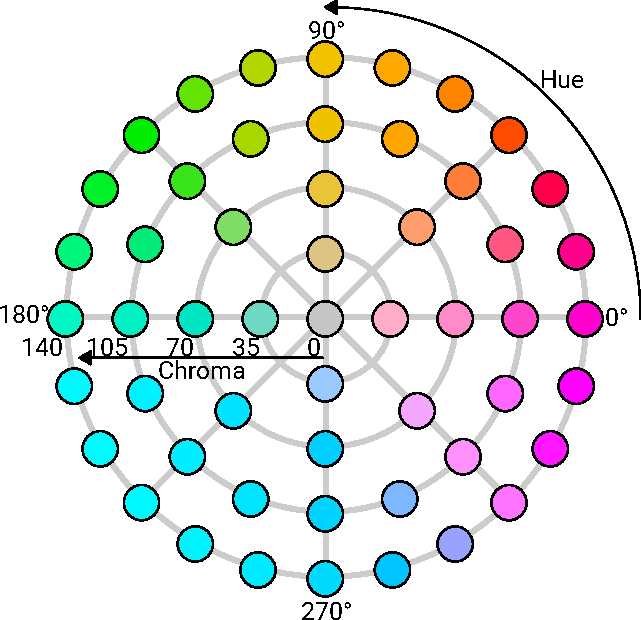
\includegraphics[width = \textwidth]{./fig/cielch.pdf}
  \subcaption{A slice of the CIE-Lch colour space with a fixed lightness $l^* = 80$ and maximum chroma $c^* = 140$.}
  \label{fig:cielch}
  \end{subfigure}%
  ~
  \begin{subfigure}[t]{0.4\textwidth}
  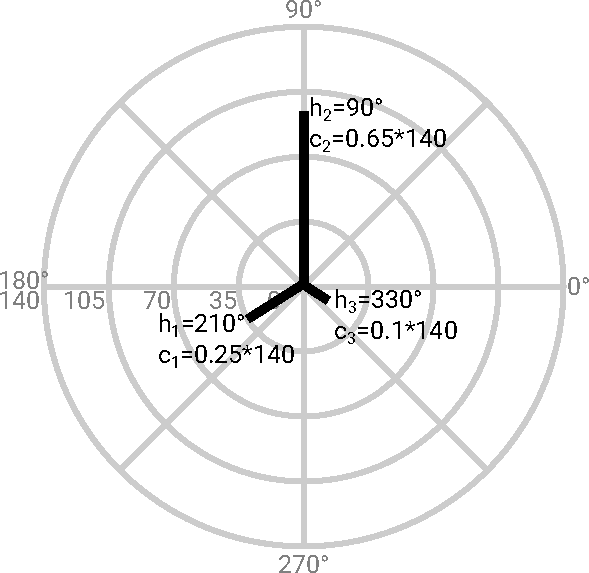
\includegraphics[width = \textwidth]{./fig/polar_vectors.pdf}
  \subcaption{Given the ternary composition $\textbf{p} = \langle 0.25, 0.65, 0.1 \rangle$ we construct three polar vectors pointing in directions $\textbf{h} = \langle 210, 90, 330 \rangle$ with magnitudes $\textbf{c} = \textbf{p}c^* = \langle 35, 91, 14 \rangle$.}
  \label{fig:polvec}
  \end{subfigure}%
  \vskip\baselineskip
  \begin{subfigure}[t]{0.4\textwidth}
  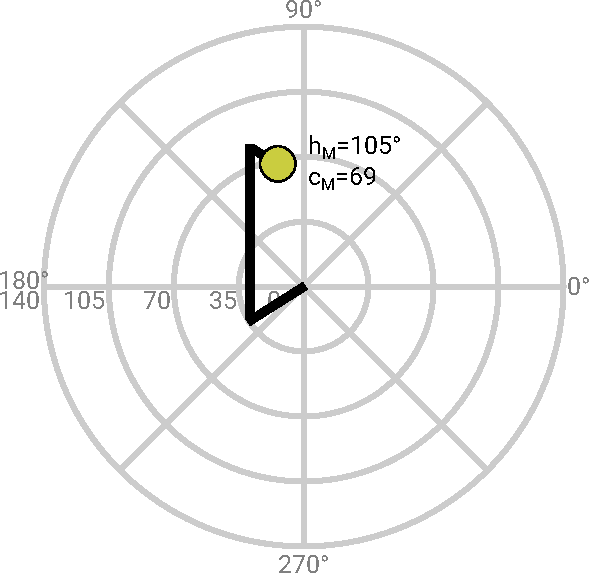
\includegraphics[width = \textwidth]{./fig/polar_vector_addition.pdf}
  \subcaption{Adding the three vectors yields the coordinates of the convex colour mixture $\mathscr{M} = \langle c = 69, h = 105 \rangle$.}
  \label{fig:poladd}
  \end{subfigure}
  ~
  \begin{subfigure}[t]{0.4\textwidth}
  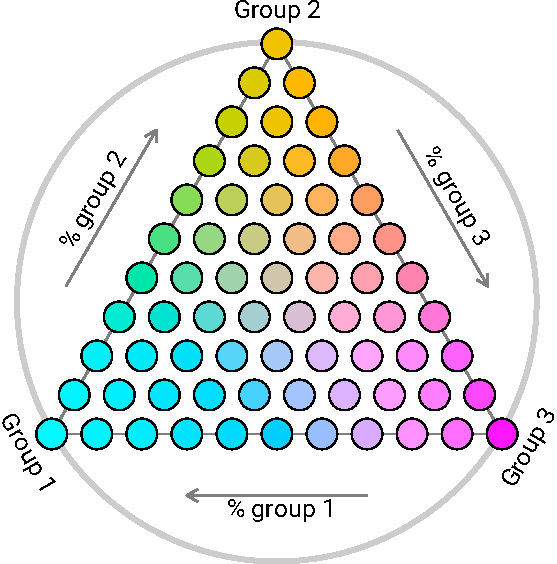
\includegraphics[width = \textwidth]{./fig/polar_ternary.pdf}
  \subcaption{The space of all possible convex colour mixtures can be shown in a ternary diagram which conveniently serves as a legend for the ternary-balance-scheme.}
  \label{fig:poltern}
  \end{subfigure}
  \caption{The ternary-balance-scheme in the CIE-Lch colour space.}
  \label{fig:tern_construction}
\end{figure}

In order to add the polar vectors we need the vector components which are given in complex form by \emph{Euler's formula}\footnote{
  Note that at this point $\textbf{h}$ has to be converted from degrees to radians. Once the colour mixture $\mathscr{M}$ is calculated, the hue parameter can be converted back into degrees.
}: $\textbf{z}=\textbf{c}\text{e}^{i \textbf{h}}$. Adding the vector components and converting back to polar coordinates gives the chroma and hue parameters of the convex colour mixture $\mathscr{M}$:

\begin{equation*}
  \mathscr{M} =
  \langle c = \text{abs}(z_1 + z_2 + z_3),
  h = \text{arg}(z_1 + z_2 + z_3) \rangle.
\end{equation*}

The colour mixtures of all possible $\textbf{p}$ form a triangular subset of the CIE-Lch slice and can be conveniently labelled with a ternary scale which allows for the numerical interpretation of each mixed-colour (see figure \ref{fig:poltern}).

\clearpage

\subsection{A discrete ternary-balance-scheme} %%%%%%%%%%%%%%%%%%%%%%%%%%%%%%%%
\label{ssec:disc}

Following \textcite{Derakhshan2009} we discretize a ternary composition $\textbf{p}$ by mapping the set of all possible ternary coordinates $P$ to a subset $P_N \subset P$ of size $N$. We perform this operation by partitioning a ternary diagram into $N$ regular triangles (regions) and mapping the ternary composition $\textbf{p}$ to the centroid coordinates $\textbf{q}$ of the region with the closest centroid. Border cases aside this is the region surrounding $\textbf{p}$.

Regions in the ternary diagram are indexed by row $j$ and row-member $i$ starting from the lower left corner. The diagram is partitioned into rows $1,\ldots,k$ and a total of $N = k^2$ regular triangles. Each row $j$ has row members $i = 1, \ldots, (2k-2j+1)$ (see figure \ref{fig:tern_quant}). The centroid coordinates $\textbf{c}$ of triangle $(j,i)$ in a ternary diagram with $k$ rows are given by

\begin{equation*}
  \textbf{c}_{ji} = \left(\frac{6k - 6j - 3i + 4 + i\mod 2} {6k},
  \frac{6j - 2 - 2 i\mod 2} {6k},
  \frac{3i - 2 + i\mod 2} {6k} \right).
\end{equation*}

To find the nearest centroid $\textbf{q}$ for a point $\textbf{p}$ we first calculate the distances between $\textbf{p}$ and all centroids $\textbf{c}_{ji}$ in the ternary diagram. The distance between points $\textbf{p}$ and $\textbf{c}$ is given by

$$
\begin{aligned}
  \textbf{l} &= \textbf{p} - \textbf{c} \\
  d(\textbf{p}, \textbf{c}) &= - l_2l_3 - l_3l_1 - l_1l_2.
\end{aligned}
$$

We return the coordinates of the centroid with the lowest distance to $\textbf{p}$.

\begin{equation*}
\textbf{q} = \underset{c_{ij}}{\text{arg\,min}}~d(\textbf{p}, \textbf{c}_{ij})
\end{equation*}

Should $\textbf{p}$ be of equal distance to multiple centroids we randomly choose among the nearest centroids. The colour mixture at the centroid coordinates is then derived as shown in appendix \ref{ssec:app-cie}.

\begin{figure}[!htb]
  \centering
  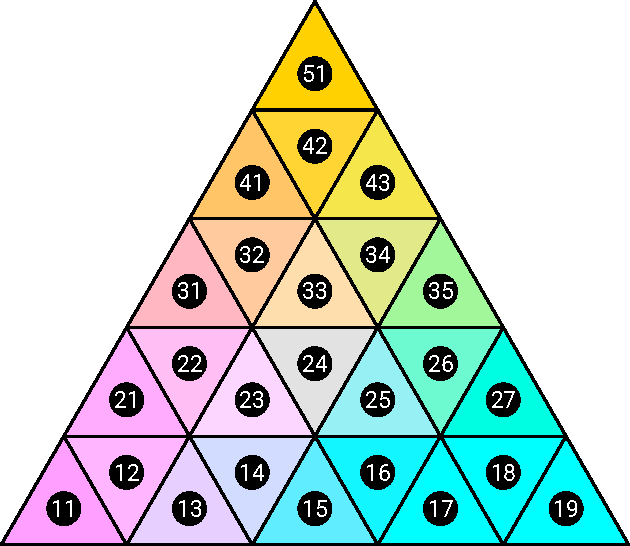
\includegraphics[width = 0.4\textwidth]{./fig/tern_quant.pdf}
  \caption{A colour coded ternary diagram with $k = 5$ rows and $N = 25$ regions. The centroid of each region is labelled with row index $j$ and entry index $i$. A ternary composition $\textbf{p}$ is discretized by mapping it to the nearest centroid.}
  \label{fig:tern_quant}
\end{figure}

\clearpage

\subsection{Increasing contrast between colours}
\label{ssec:lboost}

\begin{figure}[!htb]
\centering
  \begin{subfigure}[t]{0.3\textwidth}
  \centering
  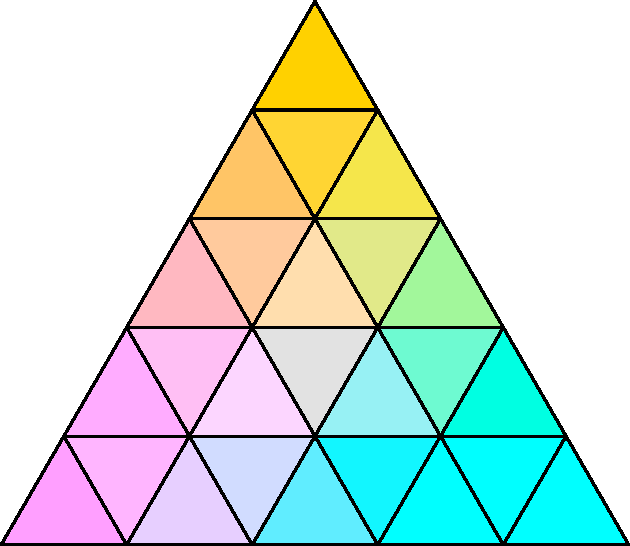
\includegraphics[width = \textwidth]{./fig/contrast0.pdf}
  \subcaption{Contrast 0.}
  \label{fig:contrast0}
  \end{subfigure}%
  ~
  \begin{subfigure}[t]{0.3\textwidth}
  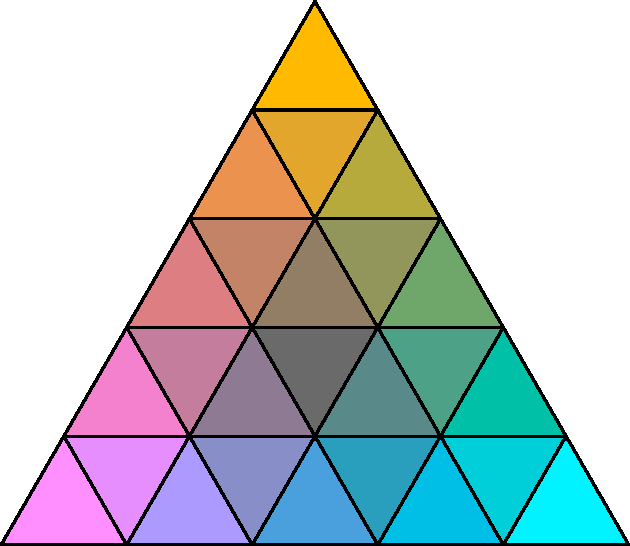
\includegraphics[width = \textwidth]{./fig/contrast0-5.pdf}
  \subcaption{Contrast 0.5.}
  \label{fig:contrast0-5}
  \end{subfigure}%
  ~
  \begin{subfigure}[t]{0.3\textwidth}
  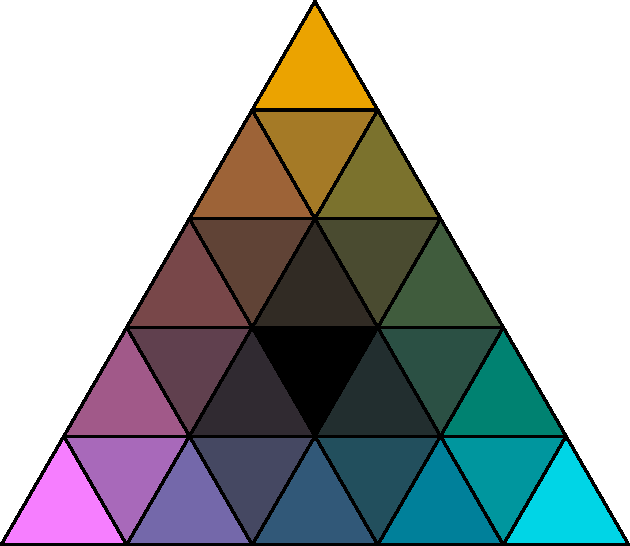
\includegraphics[width = \textwidth]{./fig/contrast1.pdf}
  \subcaption{Contrast 1.}
  \label{fig:contrast1}
  \end{subfigure}
  \caption{In order to improve the discriminability between colours in the ternary-balance-scheme we increase the lightness and chroma contrast among the mixtures. This is achieved by first rescaling chroma from range $[0, c^*]$ to $[1-\text{contrast}, 1]$ and then multiplying the lightness and chroma of mixture $\mathscr{M}$ with the rescaled chroma value to arrive at the final colour parameters. These examples have been derived from a CIE-Lch colour space with $l^*=90$, and $c^*=140$.}
  \label{fig:contrast}
\end{figure}

\clearpage

\section{Adding mortality contours to a compositional Lexis surface} %%%%%%%%%%

\setcounter{figure}{0}

\begin{figure}[!htb]
  \centering
  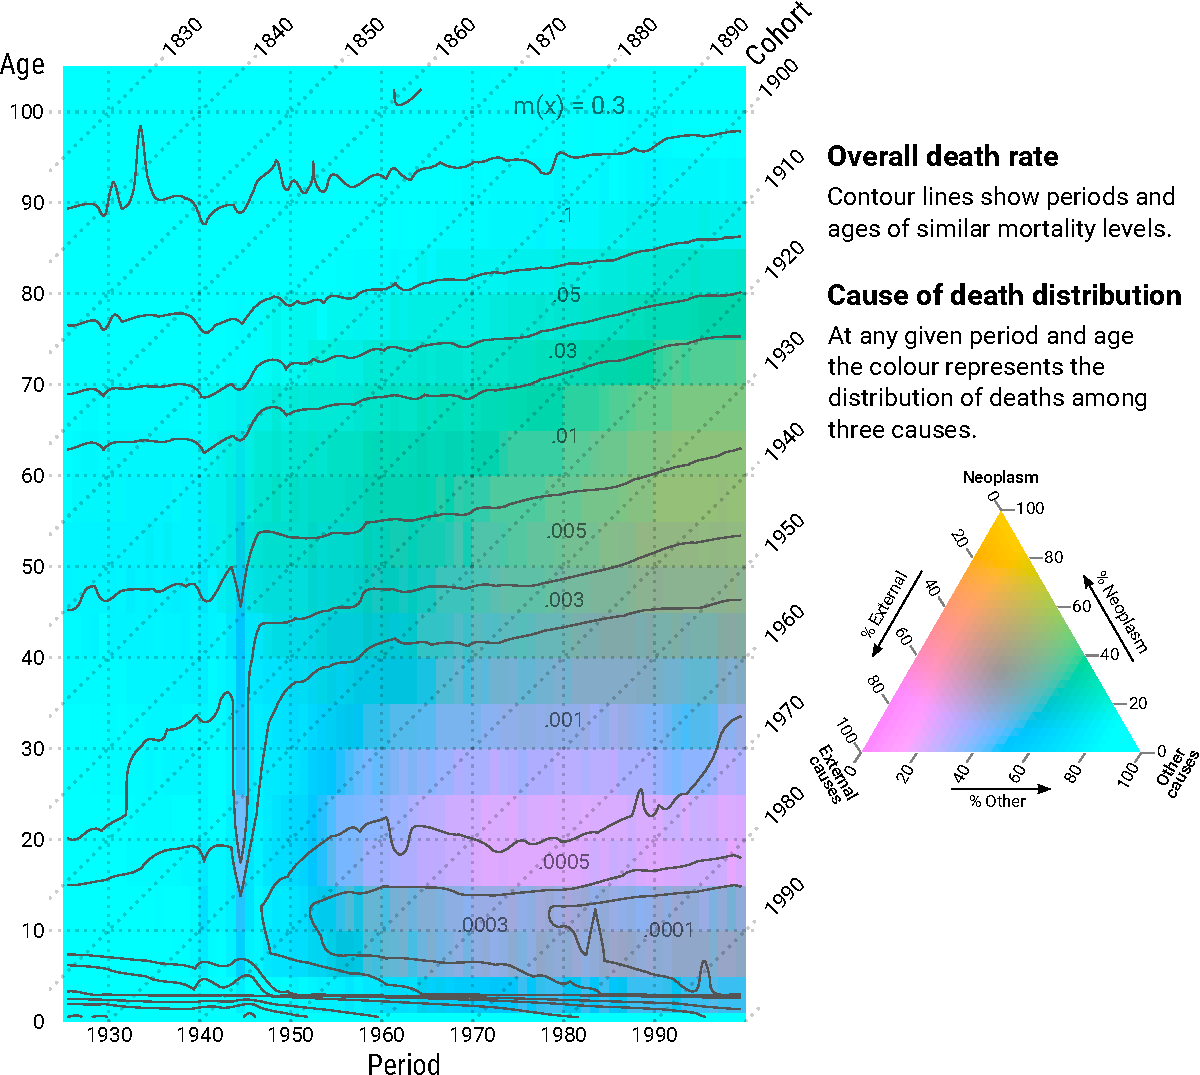
\includegraphics[width = \textwidth]{./fig/tern_balance_cont.pdf}
  \caption{The ternary-balance-scheme technique applied to French cause of death data. Age specific proportions of of people dying from a given cause in France 1925--1999, total population. We use a continuous colour-scale and overlay mortality rate contours. Data: \cite{Vallin2014}, own calculations.}
  \label{fig:tbs_cont}
\end{figure}

\end{appendix}

\end{document}